\newpage
\chapter{Machine learning}
This chapter overs generating machine learning datasets using OghmaNano. Typically you would generate these datasets then use external software such as \href{https://www.tensorflow.org/}{https://www.tensorflow.org} to perform the learning/prediction.
  
\section{Generating ML datasets}
\label{sec:machine_learning}
\subsection{Introduction}
One will often want to extract physical device parameters form a set of data using modelling. For example you may have a set of JV curves and what to extract the charge carrier mobility and recombination rate for that device.  The traditional way of doing this would be to fit a model such as OghmaNano to the data set (This is described in section \ref{sec:fitting}).  The drawback of this approach is that it can take a significant amount of time to fit one data set, furthermore when one has multiple data sets the challenge can be significant. The fitting process is complex and requires someone who is an expert in simulation with a lot of patience to perform it. This is the reason why fitting of device models to experimental data is only performed by a small subset of the community. 

A more modern approach to this problem is to use machine learning. With this approach rather than trying to fit a single JV curve, one will set up a simulation representing the device structure. However, rather than fitting the individual electrical parameters to the data set, one will generate many thousands copies of that one device but with randomly chosen electrical parameters. Each one of these devices is referred to as a \emph{virtual device}. A simulation program such as OghmaNano will then be used to generate JV curves for each of these virtual devices. Thus the user will have JV curves and the corresponding electrical parameters for each \emph{virtual device}. This data set can then be used to train a machine learning model to predict the electrical parameters from JV curves. Thus, OghmaNano is acting as a forward transform, transforming electrical parameters to simulated experimental data, then the machine learning is acting as the reverse transform that can reverse the simulation process.  Once trained this model can then be used to extract material paramters from real devices.

Advantages of this approach is that once the machine learning algorithm is trained it can extract material parameters within seconds from a device and the user does not need to be an expert at simulation to use the trained network.  However, for this method to work is key to generate a large data set on which to train the machine learning models. This process is described in the following pages.


\subsection{Generating a machine learning dataset}
This section assumes you have correctly configured your device layer structure in the layer editor. However, if you want to start with a preconfigured simulation you will be able to find this example in the New Simulation window under the \emph{ML Example}.  Figure \ref{fig:ml_main_window_device} shows the main window for a configured device, in the automation ribbon you will see a \emph{Machine learning} icon which looks like a round blue circle. If you click on this then it will open the main machine learning window show in Figure \ref{fig:main_ml_window}.

\begin{figure}
\centering
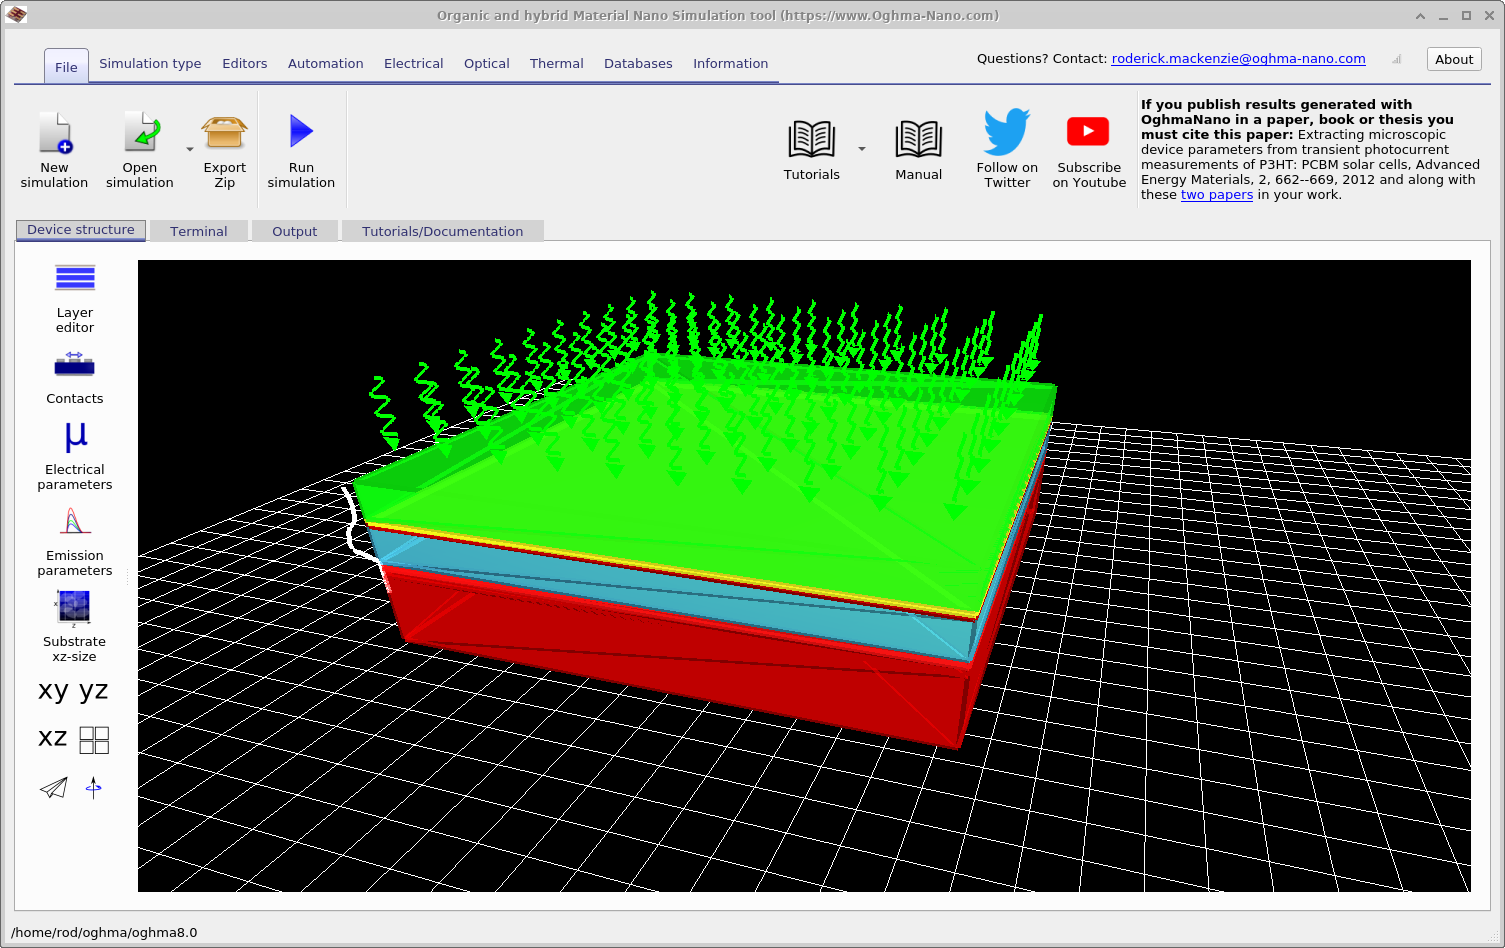
\includegraphics[width=0.5\textwidth,height=0.4\textwidth]{./images/ml/main_window.png}
\caption{The main simulation window showing the \emph{Automation} ribbon, within this ribbon the \emph{Machine learning} icon can be seen.}
\label{fig:ml_main_window_device}
\end{figure}

The main purpose of this window is to build large data sets for training machine learning algorithms. The data set we are generating is called \emph{example}.  The first tab that you can see open is called \emph{Simulations}. In this tab one defines the simulations you want performed for each \emph{virtual device}. In this case we will simulate a dark curve and 9 light curves varying between 0.0001 Suns and 1.0 Suns. The simulations can be disabled by setting \emph{Enabled} to \emph{off}.  If one clicks on the the \emph{Edit} button for the line $light\_0.0001$ in the \emph{Patch} column, the \emph{Patch window} shown in Figure \ref{fig:ml_patch} will appear. 

\begin{figure}
\centering
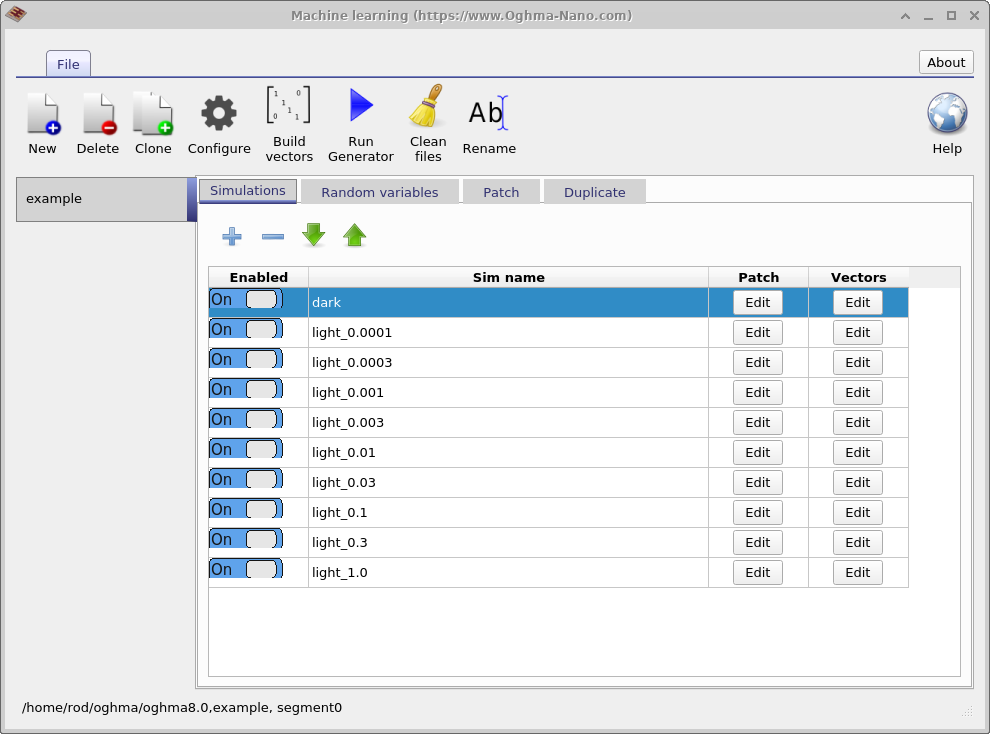
\includegraphics[width=0.9\textwidth,height=0.7\textwidth]{./images/ml/simulations.png}
\caption{The main machine learning window.}
\label{fig:main_ml_window}
\end{figure}

The purpose of the \emph{Patch window} is to change parameters in the virtual simulation. For example in our case we which to simulate a dark JV curve and nine different light intensities, therefore for each of these simulation the light intensity must be correctly adjusted. If one opens the patch window for $light\_0.0001$, you will see that the simulation variable \emph{optical/light/Psun} which controls the light intensity is set to $0.0001$. If one opens the patch window for dark, one will see that the value of \emph{optical/light/Psun} is set to $0.0$. In this way using the same base simulation multiple experiments under different conditions can be simulated.

\begin{figure}
\centering
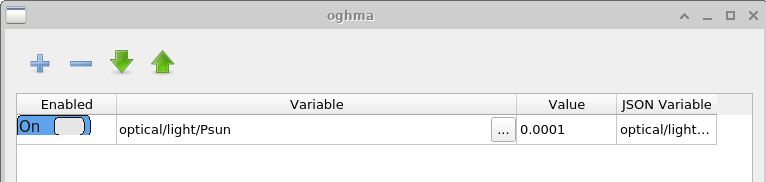
\includegraphics[width=0.9\textwidth,height=0.25\textwidth]{./images/ml/patch.png}
\caption{The simulation patch window, this window is used to change a value in a sub simulation, in this example we are changing the light intensity.}
\label{fig:ml_patch}
\end{figure}

If one now clicks on the \emph{Edit button} in the \emph{Vectors} column for the line $light\_0.0001$ in Figure \ref{fig:main_ml_window} the vectors window will appear, this is shown in Figure \ref{fig:ml_vectors}.

\begin{figure}
\centering
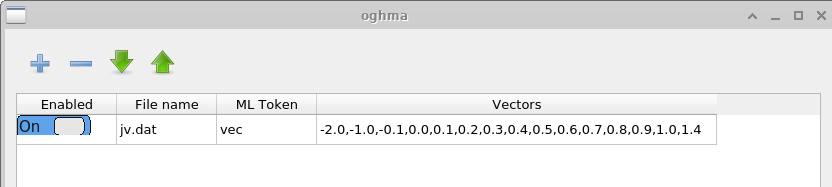
\includegraphics[width=0.9\textwidth,height=0.25\textwidth]{./images/ml/vectors.png}
\caption{The vectors window, this window defines what data is extracted from the simulation as a machine learning vector.}
\label{fig:ml_vectors}
\end{figure}

The vectors window is used to define what data is extracted from the finished simulation to act as a machine learning input vector. In this case we are extracting data points between -2.0 and 1.4 V from the file $jv.dat$, which contains the current voltage curve. If one were simulating a time domain measurement one may wish to extract various time points from the $time\_i.csv$ file or any other appropriate file. The number of points chosen to form the vector is arbitrary and up to the user. A longer input vector will make the machine learning process slower, but potentially capture more features of the JV curve.

\begin{figure}
\centering
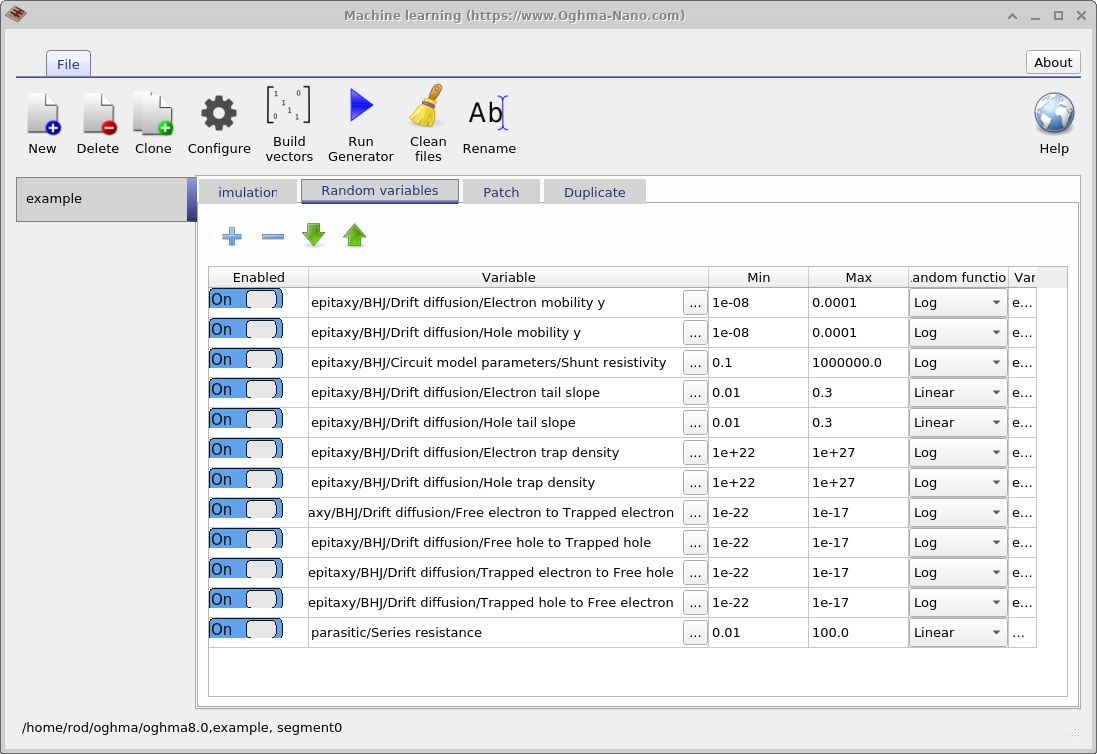
\includegraphics[width=0.9\textwidth,height=0.7\textwidth]{./images/ml/random_vars.png}
\caption{The random variables that are used for the machine learning.}
\label{fig:ml_random_vars}
\end{figure}

The next step is to set up which variables one wishes to randomize, this is done in the \emph{Random variables} tab of the main machine learning window. The window has five columns; the first column (Enabled) dictates if the random variable is used; the second column (Variable) sets which variable is changed; the third column (Min) sets the minimum allowed value of the random value; the forth column (Max) sets the maximum allowed value of the random value; and the final column (Random function) dictates if the random variable should be chosen on a log or linear scale. Log scales are recommended for variables which span multiple orders of magnitude while linear scales are recommended if the variable spans around an order of magnitude. A log distribution will ensure that an evenly distributed span of numbers are chosen across the range when viewed on a log scale. An example of a linear parameter would be Urbach energy as it typically would vary from 30 to 150 meV and example of a log variable would be trap density as it typically can vary from $1 \times 10^{15} m^{-3} - 1 \times 10^{25} m^{-3}$. 

\begin{figure}
\centering
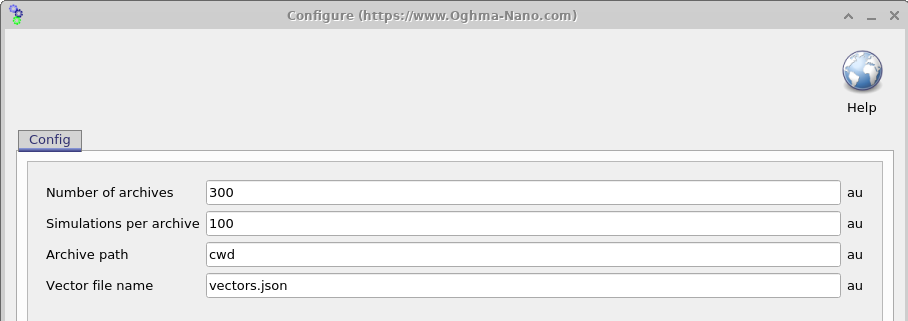
\includegraphics[width=0.9\textwidth,height=0.35\textwidth]{./images/ml/settings.png}
\caption{Configuring the data generator.}
\label{fig:ml_settings}
\end{figure}

Once the simulation has been set up, is is now time to consider how many virtual devices with randomized parameters one wishes to generate. If the \emph{Settings window} is opened, see Figure \ref{fig:ml_settings} one can configure how many \emph{virtual devices} are generated. This is controlled with two parameters, \emph{Simulations per archive} ($N_{sim}$) and \emph{Number of archives} ($N_{arc}$). These two numbers multiplied together gives you the total number of virtual devices generated. The generated simulation results are saved in zip files called \emph{archives}, each archive will contain $N_{sim}$ simulations. So in the example seen here, we will generate $N_{sim}*N_{arc}$ 3000 virtual devices stored across 100 zip files. It is important to note that for our example each virtual device will contain one dark JV curve simulation and 9 light simulations. Thus the number of files generated can quickly grow quite large. To prevent this being a problem the simulations are run in batches, with $N_{sim}$ simulations being first generated then run by OghmaNano, then stored in a zip archive until $N_{arc}$ archives are generated. In this way if the generation process is interrupted and one only looses the content of the archive currently being generated. Breaking up the data set like this also makes it easier to copy the files and more immune to corruption. Data generation will run across all CPU cores on your machine while archive generation will only run on one core.

If now the \emph{Run generator} button is pressed in the main Machine learning window Figure \ref{fig:main_ml_window}, OghamNano will start generating the simulations. After it is done, a directory called \emph{example} will appear in your simulation directory, see the left of Figure \ref{fig:ml_output_dir}. [Note to save time in this example \emph{Simulations per archive} was set to 10 and \emph{Number of archives} was set to 3]. The errors.dat file will contain any errors produced during the simulation. If one opens archive0.zip one will see the right of Figure \ref{fig:ml_output_dir}.

Each of these directories is named with a random 16 digit hexadecimal number, each directory contains an entire set of simulations for one \emph{virtual device}. So in our case each directory will contain one dark simulation and nine light simulations. The content of one of these directories is shown in the left of Figure \ref{fig:ml_archive_sim}. If one opens one of these files one can see Figure \ref{fig:ml_archive_sim} right, one can see that it contains a full OghamNano simulation. There is sim.json file there and also the jv.dat file which contains the JV curve generated during the simulation. This directory contains some extra data including optical outputs and a cache file. It is recommended to try to minimize all output when generating these files otherwise the total size on disk becomes very large, this can be done by turning all the output verbosity options to produce minimal output. 

\begin{figure}
\centering
\begin{tabular}{ c c }

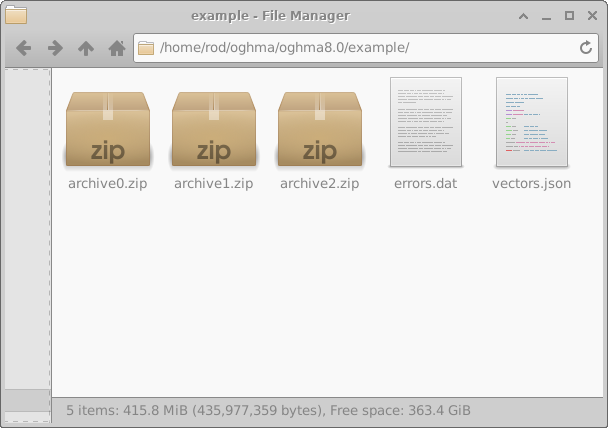
\includegraphics[width=0.5\textwidth,height=0.4\textwidth]{./images/ml/output_dir.png}

&
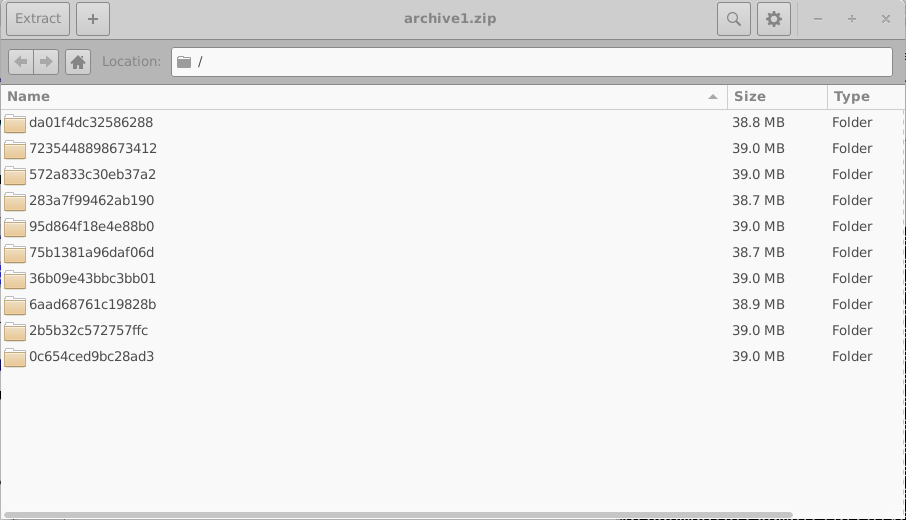
\includegraphics[width=0.5\textwidth,height=0.4\textwidth]{./images/ml/zipfile.png}
\\
\end{tabular}
\caption{Left: The content of the \emph{Example} directory; Right inside archive0.zip}
\label{fig:ml_output_dir}
\end{figure}


In the above example we only have three archives but in a normal simulation run one would have up to 200 archives each with 200 simulations in each. Once the simulations have been performed one needs to convert these raw OghmaNano simulations into a vectors file for the machine learning algorithm.  If one clicks on the \emph{Build vectors} icon in the main machine learning window \ref{fig:main_ml_window}, OghamNano will open each virtual simulation and compile the it to a vectors file. The vectors file can be seen in Figure \ref{fig:ml_vectors_file}. 

\begin{figure}
\centering
\begin{tabular}{ c c }

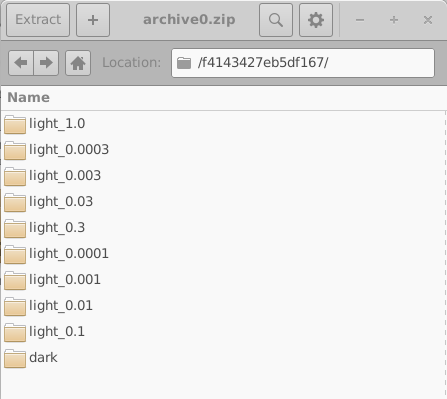
\includegraphics[width=0.5\textwidth,height=0.4\textwidth]{./images/ml/archive_sims.png}

&
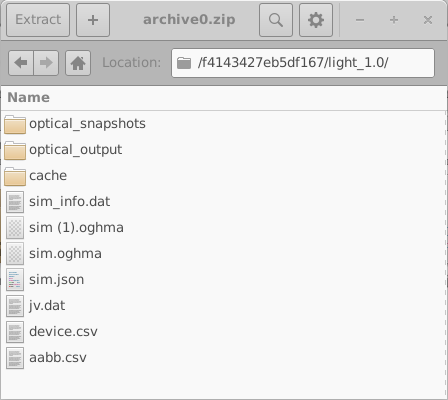
\includegraphics[width=0.5\textwidth,height=0.4\textwidth]{./images/ml/archive_sim.png}
\\
\end{tabular}
\caption{Left: The content of the \emph{Example} directory; Right inside archive0.zip}
\label{fig:ml_archive_sim}
\end{figure}

This vectors file is a json file containing all the data needed for training a machine learning algorithm. Each \emph{virtual device} in the data set will have a section in the file. So for example in this figure we are looking at the section relating to device 2cbd08c0fd7eb406 (line 3), we can see under the heading \emph{params} what electrical parameters were randomly chosen for this device. Followed by the vectors representing the dark JV curve (line 19) and the light JV curve at 0.0001 Suns (line 22). These values in this example are in $Am^{-2}$, however they will always be the same as the file from which they are extracted. So in this case jv.dat contains Volts v.s. $Am^{-2}$ therefore the values of the vector are $Am^{-2}$. After this key device parameters such as PCE are dumped. There will be one entry in this file for each virtual device generated. Once you have this file, you can feed it into the machine learning algorithm of your choice. Some users report that it is easier to feed this data into tensor flow if it is first converted into a CSV file, this can be done using the standard Python libraries.

\begin{figure}
\centering
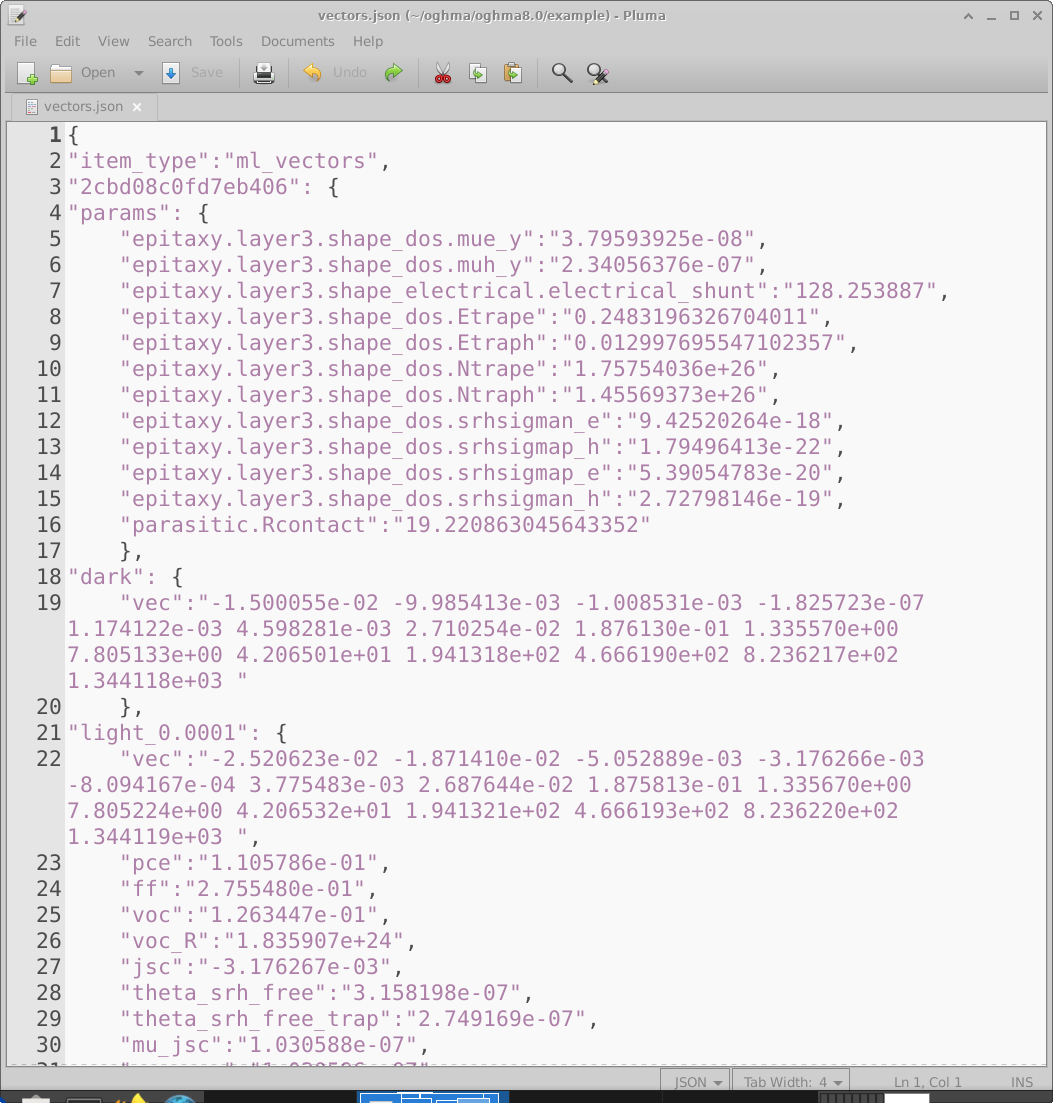
\includegraphics[width=\textwidth,height=1.0\textwidth]{./images/ml/output.png}
\caption{The final vectors file in json format. This file can be fed into machine learning model as a training set.}
\label{fig:ml_vectors_file}
\end{figure}

\subsection{Setting up machine learning algorithms to process the data}
The above section describes how to generate machine learning data sets. Setting up the algorithm it's self is a large topic on it's own. However there are many good examples at \href{https://www.tensorflow.org/}{https://www.tensorflow.org/}.
